\documentclass[11pt,a4paper]{article}
\usepackage{amsmath,amssymb,graphicx,geometry,booktabs,hyperref,longtable}
\usepackage{setspace}
\onehalfspacing
\emergencystretch=3em
\geometry{margin=1in}

\title{\textbf{Optimal WTI---FX Hedge Ratios Under a Fixed Budget:\\ A Maturity-Matched Strip Program with a Tail Objective}}
\author{\textbf{Jihong Park} \\ Pusan National University \\ \texttt{adrianus026@gmail.com}}
\date{August 2026}

\begin{document}

\maketitle

\begin{abstract}
A Korean crude-oil importer facing correlated WTI and USD/KRW exposure must decide, before any option is bought, what fraction of each exposure to hedge out of a fixed spending authority, in which instrument, and at what maturity. This paper formulates the decision as a maturity-matched strip program: each of the next twelve monthly procurement lots is covered by options expiring at its own settlement date, so a monthly authority of KRW 45bn aggregates to an annual strip authority of KRW 540bn with no overlap between tranches. The risk objective is the conditional value-at-risk of the strip's simulated loss distribution under the calibrated jump-diffusion, solved by the Rockafellar---Uryasev program and verified on a deterministic grid. Four results follow. First, maturity matching itself is worth KRW 95.3bn per year: the matched strip prices full WTI coverage at KRW 399.8bn against KRW 495.1bn for twelve uniform ten-month contracts. Second, under a tail objective the WTI leg, which settles at the realized exchange rate, covers the joint tail on its own: with one coverage envelope ($w_1+w_2\le1$) the CVaR$_{95}$ optimum is the corner $(1,0)$ and the authority is slack, while with separate books ($\kappa=2$) the authority binds exactly, pinning FX coverage at $w_2=0.836$ with a shadow price of KRW 2.6bn of CVaR$_{95}$ per billion of authority. Third, the currency leg belongs at the same maturity as the barrels it converts: capping the FX slices at half a year saves at most KRW 14bn of premium and spread under a bid-ask curve that steepens as fast as linearly in tenor, and costs KRW 77bn of CVaR$_{95}$, so co-termed slices dominate throughout the examined spread range. Fourth, the instrument question: a knock-out structure's premium discount is priced against its own stress mortality, measured by re-simulation from the stress state at $49\%$ for the contract actually held, an order of magnitude above the closed-form indifference mortality of $4.24\%$ at which the discount stops paying for itself; the mixed vanilla/knock-out program therefore selects the all-vanilla book at no cost in residual risk.
\end{abstract}

\vspace{0.5em}
\noindent\textbf{Keywords:} corporate hedging; hedge ratio; conditional value-at-risk; option strip; knock-out barrier; commodity and currency risk; budget constraint

\vspace{0.3em}
\noindent\textbf{JEL classification:} G32; G13; Q40; C61

\tableofcontents
\newpage

\section{Introduction}

Before a hedging desk debates \emph{how} to run an option hedge (which pricing model, which rebalancing rule, which Greeks) the treasurer must answer three cruder questions: out of a fixed hedging budget, \emph{what fraction of each exposure should be covered}, \emph{with which instrument}, and \emph{at which maturities}? For a Korean crude-oil importer the exposures are two: the WTI price of the physical barrels it buys every month, and the USD/KRW exchange rate at which the resulting dollar liability is converted into won. In the configuration studied here the physical requirement is 2{,}000{,}000 barrels per month, the equivalent dollar need is \$157{,}880{,}000 per month, and the option authority is KRW 45{,}000{,}000{,}000 per month.

A monthly authority and a multi-month option cannot be reconciled one contract at a time: a single long-dated contract bought each month produces overlapping tranches whose combined premium has no monthly ledger. The program studied here removes the mismatch at its source. The decision object is a \emph{strip}: for each of the next twelve monthly procurement lots $m=1,\dots,12$, the desk buys options expiring at that lot's own settlement date $T_m=m/12$. Coverage is uniform across slices, so the decision variables remain two scalars: $w_1\in[0,1]$, the fraction of each month's WTI exposure covered by WTI calls of matching maturity, and $w_2\in[0,1]$, the fraction of each month's USD need covered by USD/KRW calls of matching maturity. The monthly authority aggregates to an annual strip authority $12B=$ KRW 540bn against the strip's total premium, and in steady state the rolling implementation spends one slice's premium per month. Nothing overlaps, and the budget governs exactly the cash the desk pays.

The risk objective is the tail of the strip's loss distribution. Losses are simulated under the calibrated jump-diffusion on the physical measure, and the program minimizes the conditional value-at-risk at the $95\%$ level (Rockafellar and Uryasev, 2000), a coherent risk measure in the sense of Artzner et al.\ (1999). A single-scenario stress ledger and the classical variance objective are computed alongside for comparison, on the same path bank.

Four questions organize the paper. (a) \textbf{Does the annual authority bind?} (b) \textbf{What mechanism produces the extreme $w_1/w_2$ asymmetry} that variance-based programs exhibit, and does a tail objective preserve it? (c) \textbf{At which maturity does the currency leg belong}, given that FX option bid-ask spreads widen with tenor? (d) \textbf{Does a knock-out structure's premium discount survive its own mortality?} The answers, previewed. (a) Under one coverage envelope ($w_1+w_2\le1$) the authority is slack: the most expensive feasible book, full WTI coverage, costs KRW 399.8bn against KRW 540bn. Under separate books ($w_1+w_2\le2$) the authority binds exactly, pins FX coverage at $w_2=0.836$, and carries a shadow price of KRW 2.6bn of CVaR$_{95}$ per billion of authority up to the full-coverage premium of KRW 567.5bn. (b) The variance asymmetry is structural, a closed-form consequence of an 18-to-1 variance ratio at near-zero correlation; the tail objective sharpens it to a corner, because the WTI leg settles at the realized exchange rate and therefore covers the joint tail by itself. (c) Co-termed: capping the FX slices at half a year costs five to twelve times more tail than it saves in premium and spread under any plausible spread term structure. (d) No: measured by re-simulation from the stress state, the contract actually held is dead on $49\%$ of the paths that reach the scenario it was bought against, eleven times the closed-form indifference mortality, and the mixed vanilla/knock-out program of Section~\ref{sec:mixed} selects the all-vanilla book.

\section{Literature Review}

The variance benchmark is the classical minimum-variance portfolio criterion of Markowitz (1952), specialized to two residual exposures: the quantity minimized is the standard deviation of a two-asset portfolio whose weights are the \emph{unhedged} fractions $(1-w_1)$ and $(1-w_2)$. The closed-form line-restricted solution used in Section~\ref{sec:asymmetry} is the textbook two-asset global-minimum-variance weight, and its unconstrained special case is the minimum-variance hedge ratio of Ederington (1979). The tail objective is the conditional value-at-risk of Rockafellar and Uryasev (2000), coherent in the sense of Artzner et al.\ (1999); the optimization exploits their linearizable auxiliary formulation directly on the simulated path bank.

The premium inputs come from two closed-form option models applied slice by slice. Black (1976) prices each WTI slice as a call on the commodity forward; Garman and Kohlhagen (1983) price each FX slice as a currency call with separate domestic and foreign interest rates. The knock-out analysis of Sections~\ref{sec:pko}--\ref{sec:mixed} prices the barrier structure by Longstaff---Schwartz (2001) least-squares Monte Carlo under jump-diffusion dynamics in the spirit of Merton (1976); the diffusive volatility $0.3242$ that valuation consumes is what a threshold-classification jump/diffusion decomposition leaves after stripping the jump variance out of the raw historical volatility $0.3946$, and it is an input to the pricing engine and not to the risk objective, which takes the raw figure because the uncovered barrels bear the jumps as well as the diffusion. Because the barrier structure prices both legs jointly, its premium is attributed to individual legs by Shapley (1953) value where a per-leg report is needed; Section~\ref{sec:split} establishes what that attribution can and cannot identify.

The economic question (how much of each of two correlated exposures to cover when hedging is costly) descends from the cross-hedging literature of Anderson and Danthine (1981) and, for the currency dimension of internationally sourced commitments, Adler and Dumas (1984). The present setting differs from the classical futures cross-hedge in one decisive respect: hedging is done with options bought under a hard spending authority, so the operative trade-off runs between a tail measure and an explicit cap on premium cash, in place of the usual variance/expected-return frontier. The closest instrument-level antecedent is Ahn, Boudoukh, Richardson, and Whitelaw (1999), who optimize a put-option hedge under an explicit premium constraint and characterize the strike that buys the most value-at-risk reduction per dollar of cost; the present program shares their premium-constrained logic but allocates one budget across two correlated exposures and twelve maturities with the contracts held fixed. Brown and Toft (2002) solve the complementary problem, deriving the firm's optimal customized payoff under joint price and quantity risk; here the payoffs are given market instruments, which is what makes the question an allocation rather than a design problem.

The premium budget is taken as exogenous, following the corporate hedging literature that supplies its rationale. Rampini, Sufi, and Viswanathan (2014) derive hedging bounded by collateral and financing capacity rather than chosen at an unconstrained optimum, which is the mechanism a spending authority proxies for; Campello, Lin, Ma, and Zou (2011) document the financing frictions empirically, and P\'erez-Gonz\'alez and Yun (2013) and Gilje and Taillard (2017) supply identification-based evidence that hedging affects value. Froot, Scharfstein, and Stein (1993) model the institutional friction: a firm hedges to protect its internal financing capacity for investment and not to maximize variance reduction per se, which is consistent with hedging being bounded by an approved cash outlay. Stulz (1996) develops the practitioner-facing corollary that selective, partial hedging can be optimal even when full coverage is affordable, the same qualitative conclusion Section~\ref{sec:asymmetry} reaches by a purely variance-arithmetic route. Jin and Jorion (2006) document derivative-based hedging behavior among U.S.\ oil and gas producers; the importer studied here sits on the opposite side of the same commodity risk.

\section{The Strip Allocation Program}
\label{sec:problem}

\subsection{Slices, Notionals, and Decision Variables}

Month $m$'s procurement lot is $Q_{oil}=2{,}000{,}000$ bbl settled at $T_m=m/12$, $m=1,\dots,12$. At the calibration spot the barrel requirement and the dollar requirement of each lot are the same quantity of money,
\begin{equation}
Q_{oil}\cdot S_{WTI} \;=\; 2{,}000{,}000 \times 78.94 \;=\; \$157{,}880{,}000 \;=\; Q_{USD},
\label{eq:notionalidentity}
\end{equation}
so a barrel hedged and a dollar hedged cover the identical underlying cash outflow, once through its price and once through its currency of settlement. Slice $m$ carries a WTI call on $w_1 Q_{oil}$ barrels and a USD/KRW call on $w_2 Q_{USD}$ dollars, both expiring at $T_m$; coverage $(w_1,w_2)$ is uniform across slices. Strikes follow the production configuration, $5\%$ in the money on both legs: $K_1=0.95\,S_{WTI}=74.99$ USD/bbl and $K_2=0.95\,S_{KRW}=1{,}463.61$ KRW/USD.

The coverage envelope is $w_1+w_2\le\kappa$. At $\kappa=1$ the two legs share one notional envelope: a treasury that authorizes hedging of ``the monthly crude bill'' and treats $w_1$ and $w_2$ as two ways of covering that one bill, in the sense of \eqref{eq:notionalidentity}, imposes exactly this. At $\kappa=2$ the price book and the currency book are separate, each hedgeable up to its own notional. Both designs are solved throughout, because Section~\ref{sec:results} shows the answer to question~(a) is the choice between them.

\subsection{Premiums and the Authority}
\label{sec:cost}

Slice $m$'s premiums are closed-form at its own maturity: $P_{B76}(T_m)$ per barrel (Black-76 on the flat forward at the historical volatility $\sigma_1=0.3946$) and $P_{GK}(T_m)$ per dollar (Garman---Kohlhagen at $\sigma_2=0.0926$). Premium cash is carried to each slice's settlement on the funding factor $(1+r_w T_m)$ with $r_w=0.07$. The strip's premium is affine in the coverage pair,
\begin{equation}
\Pi(w_1,w_2) \;=\; w_1\underbrace{\sum_{m=1}^{12} Q_{oil}\,P_{B76}(T_m)\,S_{KRW}\,(1+r_wT_m)}_{K_1^S\;=\;\text{KRW 399.75bn}}
\;+\; w_2\underbrace{\sum_{m=1}^{12} Q_{USD}\,P_{GK}(T_m)\,(1+r_wT_m)}_{K_2^S\;=\;\text{KRW 167.74bn}},
\label{eq:strippremium}
\end{equation}
and the budget constraint is the cash constraint
\begin{equation}
\Pi(w_1,w_2)\;\le\;12B\;=\;\text{KRW }540{,}000{,}000{,}000.
\label{eq:authority}
\end{equation}
Full coverage of both legs costs $K_1^S+K_2^S=$ KRW 567.5bn, $5.1\%$ above the authority, so the affordable set excludes a corner neighborhood of $(1,1)$ and nothing else.

Maturity matching is itself a first-order economy. Twelve uniform contracts at the production tenor $T=0.833$ would price full WTI coverage at $12\times$ KRW 41.26bn $=$ KRW 495.1bn; the matched strip prices it at KRW 399.8bn. The difference, KRW 95.3bn per year or $19.3\%$ of the uniform-tenor premium, is the cost of buying ten months of optionality for exposures that settle in one to nine, and the strip eliminates it by construction.

\subsection{Risk Objectives}
\label{sec:objectives}

Three risk metrics are evaluated on one simulated path bank; the first is the program's objective.

\emph{Tail objective.} With $S_1^{(m)},S_2^{(m)}$ the simulated prices at $T_m$, the strip's loss relative to inception procurement cost is affine in the coverage pair path by path,
\begin{align}
L(w_1,w_2) \;&=\; A \;-\; w_1\,B^{\mathrm{WTI}} \;-\; w_2\,C^{\mathrm{FX}},
\label{eq:loss}\\
A \;&=\; \sum_m Q_{oil}\bigl(S_1^{(m)}S_2^{(m)}-S_1(0)S_2(0)\bigr), \nonumber\\
B^{\mathrm{WTI}} \;&=\; \sum_m Q_{oil}\bigl(S_1^{(m)}-K_1\bigr)^{+}S_2^{(m)}, \qquad
C^{\mathrm{FX}} \;=\; \sum_m Q_{USD}\bigl(S_2^{(m)}-K_2\bigr)^{+}, \nonumber
\end{align}
and the program is
\begin{equation}
\min_{w_1,w_2}\ \mathrm{CVaR}_{0.95}\bigl[L(w_1,w_2)\bigr]
\quad\text{s.t.}\quad \Pi(w_1,w_2)\le 12B,\qquad w_1+w_2\le\kappa,\qquad w\in[0,1]^2.
\label{eq:program}
\end{equation}
Because $L$ is affine in $(w_1,w_2)$ path by path, its CVaR is convex in $(w_1,w_2)$ and every constraint is affine: any local minimum of \eqref{eq:program} is global. The WTI term in \eqref{eq:loss} carries the realized exchange rate $S_2^{(m)}$ because the barrel calls settle in dollars converted at expiry; that single fact drives the tail geometry of Section~\ref{sec:tail}.

\emph{Variance benchmark.} The classical residual standard deviation
\begin{equation}
\sigma_{res}(w_1,w_2) \;=\; \sqrt{(1-w_1)^2\sigma_1^2 + (1-w_2)^2\sigma_2^2 + 2(1-w_1)(1-w_2)\,\sigma_1\sigma_2\rho}\,,
\label{eq:gmvp}
\end{equation}
with $\sigma_1=0.3946$, $\sigma_2=0.0926$, $\rho=0.0876$: the volatility of what is left uncovered, which does not know which model priced its hedge.

\emph{Stress ledger.} The annualized single-scenario ledger prices the unhedged fraction at (WTI 113, USD/KRW 1550): $UL_1=12\,Q_{oil}\max(0,113-78.94)\times1550=$ KRW 1{,}267.0bn and $UL_2=12\,Q_{USD}\max(0,1550-1540.64)=$ KRW 17.7bn at full openness. It is reported as a scenario diagnostic alongside the distributional objective, and it is the ledger on which the knock-out mortality of Section~\ref{sec:pko} is priced, because barrier death is a scenario-conditional event.

\subsection{Identification of the Premium Split}
\label{sec:split}

Sections~\ref{sec:pko}--\ref{sec:mixed} price a jointly-written barrier structure, and reporting its single premium leg by leg requires an attribution. The Shapley construction prices $v(\{1\})$ by freezing the currency volatility and $v(\{2\})$ by freezing the WTI dynamics. For this payoff the first operation does nothing. A change-of-numeraire factorization of the composite payoff shows the structure's value is $S_2(0)e^{-r_{US}T}\,\mathbb E^{Q_{US}}[X(T)]$, in which neither $\sigma_2$ nor $\rho$ appears, so
\begin{equation}
v(\{1\}) \;=\; v(\{1,2\}) \qquad\text{exactly, and hence}\qquad \phi_{FX} \;=\; \tfrac12\,v(\{2\}),
\label{eq:degenerate}
\end{equation}
half the value of the structure with WTI frozen: a deterministic intrinsic-value quantity containing no FX optionality. The pricing engine confirms the degeneracy directly: at $100{,}000$ paths over two seeds, $v(\{1,2\})-v(\{1\})$ is $77$--$97$ KRW per unit against a Monte Carlo standard error of $63$ and a premium near $17{,}100$, and $\phi_{FX}$ sits within $50$ KRW of $\tfrac12 v(\{2\})$. The joint premium has no FX-volatility component to attribute, and the Shapley axioms cannot conjure one.

Two consequences govern how the attribution is used. Any quantity evaluated where the two ratios move together is convention-invariant, the joint premium total in particular. Every \emph{marginal} per-leg statement is convention-dependent, which is why the instrument decisions of Section~\ref{sec:mixed} are made on standalone, separately-traded instrument prices and not on the attribution.

\section{Calibration}
\label{sec:data}

Table \ref{tab:inputs} lists every input. The underlying series are daily WTI spot (USD/bbl) and USD/KRW, covering 28 June 2021 to 22 June 2026, 1{,}301 paired closing observations retained after aligning the two calendars. Differencing gives 1{,}300 paired daily log returns, of which 1{,}299 survive the jump-classification screen and constitute the estimation sample: $\sigma_1 = 0.3946$ (WTI, annualized), $\sigma_2 = 0.0926$ (USD/KRW), $\rho = 0.0876$. The diffusive volatility $\sigma_1^{diff}=0.3242$ and the symmetrized Merton triple $(\lambda,\theta_J,\delta_J)=(6.7846,\,-0.0299,\,0.08443)$ come from the threshold-classification jump/diffusion decomposition of the same series: jump days are identified by a $k$-sigma rule, the two jump regimes are moment-matched, and the diffusive volatility is re-estimated from the remainder, so the observed variance is split rather than duplicated.

The loss simulation runs on the physical measure: WTI follows the jump-diffusion at $\sigma_1^{diff}$ with the symmetrized jump triple, compensator in the drift, and physical drift $\mu_1=0.139$ (the sample mean); USD/KRW follows a correlated geometric Brownian motion at $\sigma_2$ with baseline drift $\mu_2=0$, the flat-forward convention, with the uncovered-interest-parity drift $r_{KRW}-r_{US}=-0.005$ as a robustness variant (Section~\ref{sec:robust}). The bank holds $200{,}000$ paths on the monthly settlement grid under a fixed seed; premiums, by contrast, are closed-form and consume no simulation.

The FX bid-ask spread term structure of Section~\ref{sec:fxmat} is parameterized as
\begin{equation}
s(T) \;=\; s_{1M}\,(12\,T)^{\gamma}\quad\text{vol points},
\label{eq:spread}
\end{equation}
anchored at the one-month tenor and steepening with $\gamma$; options are bought at mid plus half-spread. The grid spans $s_{1M}\in\{0.2,0.4,0.8\}$ vol points and $\gamma\in[0.1,1.2]$, which spans tight to wide spread conditions: at $s_{1M}=0.8,\ \gamma=1.0$ the one-year spread is $9.6$ vol points, and the conclusion of Section~\ref{sec:fxmat} is settled well before that point.

\begin{table}[h]
\centering
\small
\begin{tabular}{llr}
\toprule
Quantity & Symbol & Value \\
\midrule
WTI spot (USD/bbl) & $S_{WTI}$ & 78.94 \\
USD/KRW spot & $S_{KRW}$ & 1{,}540.64 \\
Monthly oil need (bbl) & $Q_{oil}$ & 2{,}000{,}000 \\
Monthly USD need & $Q_{USD}$ & 157{,}880{,}000 \\
WACC (funding rate) & $r_w$ & 0.07 \\
Monthly authority (KRW) & $B$ & 45{,}000{,}000{,}000 \\
Annual strip authority (KRW) & $12B$ & 540{,}000{,}000{,}000 \\
Strip slice maturities (yr) & $T_m$ & $m/12,\ m=1,\dots,12$ \\
WTI call strike (USD/bbl) & $K_1 = 0.95\,S_{WTI}$ & 74.99 \\
FX call strike (KRW/USD) & $K_2 = 0.95\,S_{KRW}$ & 1{,}463.61 \\
Knock-out call strike (USD/bbl) & $K = S_{WTI}$ & 78.94 \\
Knock-out barriers (USD/bbl) & $U$, $L$ & 120, 50 \\
Stress WTI (USD/bbl) & $S^{st}_{WTI}$ & 113 \\
Stress USD/KRW & $S^{st}_{KRW}$ & 1{,}550 \\
WTI volatility, risk objective & $\sigma_1$ & 0.3946 \\
WTI diffusive vol, simulation and pricing & $\sigma_1^{diff}$ & 0.3242 \\
USD/KRW vol & $\sigma_2$ & 0.0926 \\
WTI---FX correlation & $\rho$ & 0.0876 \\
WTI physical drift & $\mu_1$ & 0.139 \\
FX physical drift (baseline) & $\mu_2$ & 0 \\
USD risk-free rate (pricing) & $r_{US}$ & 0.040 \\
KRW risk-free rate (pricing) & $r_{KRW}$ & 0.035 \\
Jump intensity (symmetrized) & $\lambda$ & 6.7846 /yr \\
Mean jump size (log) & $\theta_J$ & $-0.0299$ \\
Jump volatility (log) & $\delta_J$ & 0.08443 \\
CVaR level & $\alpha$ & 0.95 \\
FX spread anchor (vol points, 1M) & $s_{1M}$ & 0.2 / 0.4 / 0.8 \\
FX spread steepness & $\gamma$ & 0.1 -- 1.2 \\
\bottomrule
\end{tabular}
\caption{Model inputs. The risk block is estimated from the price history of Section~\ref{sec:data}; the jump block and the two pricing rates enter the simulation and the knock-out analysis of Sections~\ref{sec:pko}--\ref{sec:mixed}. Every downstream number in this paper is computed from these values; the slice-level premiums generated from them are plotted in Figure~\ref{fig:strippremium}.}
\label{tab:inputs}
\end{table}

\begin{figure}[h]
\centering
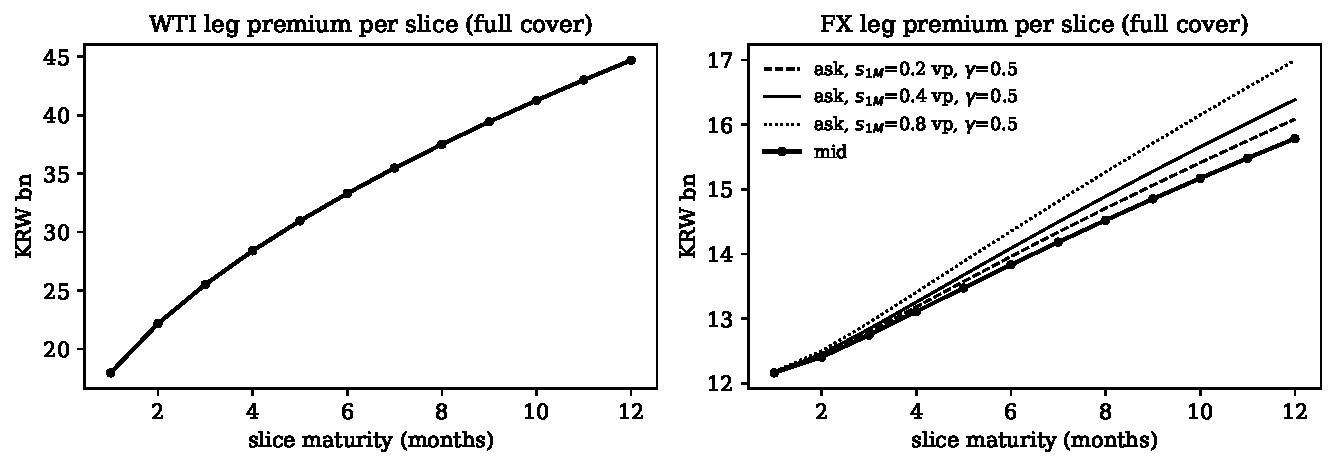
\includegraphics[width=\textwidth]{figures/fig_strip_premium.pdf}
\caption{Per-slice full-coverage premiums across the twelve strip maturities. Left: WTI leg (Black-76 at each slice's tenor, funded). Right: FX leg (Garman---Kohlhagen mid, funded), with ask curves under the spread term structure \eqref{eq:spread} at $\gamma=0.5$. The strip totals are the coefficients of \eqref{eq:strippremium}: KRW 399.75bn and KRW 167.74bn.}
\label{fig:strippremium}
\end{figure}

\section{Numerical Method and Verification}
\label{sec:method}

The premium map \eqref{eq:strippremium} and both constraint sets are affine, and $\mathrm{CVaR}_\alpha[L(w)]$ is convex in $w$ because $L$ is affine in $w$ path by path; every program solved in this paper is therefore convex, and any local minimum is the global minimum.

The tail program \eqref{eq:program} is solved in the Rockafellar---Uryasev auxiliary form: with $t$ the value-at-risk variable,
\begin{equation}
\mathrm{CVaR}_\alpha[L(w)] \;=\; \min_t\ t + \frac{1}{(1-\alpha)N}\sum_{i=1}^N \bigl(L_i(w)-t\bigr)^+,
\label{eq:ru}
\end{equation}
minimized jointly over $(w_1,w_2,t)$ by SLSQP from five starting points on the $200{,}000$-path bank. Every reported optimum is cross-checked against an exhaustive deterministic grid ($41$ points per axis, empirical tail mean at each node): at $\kappa=1$ the two methods return the identical corner; at $\kappa=2$ the grid's best node differs from the SLSQP optimum by one grid spacing in $w_2$, because the budget-pinned optimum $w_2=0.836$ falls between grid nodes, and the SLSQP value is the lower of the two. The variance and stress-ledger programs are solved with the same multi-start SLSQP machinery. Closed-form premiums are verified against the production engine at the overlapping tenors: the $T=0.833$ Black-76 slice reprices to \$12.6524 and the $T=0.5$ Garman---Kohlhagen slice to KRW 84.667, both reproducing the engine to the displayed digits.

The scenario-conditional knock-out probability of Section~\ref{sec:pko} is measured by direct simulation of the calibrated WTI jump-diffusion started \emph{at the stress spot} and monitored against the 120/50 barriers with jump-adapted exact first-passage sampling: Poisson jump times are drawn exactly within each daily step, the Brownian-bridge crossing probability is applied on each jump-free sub-interval, and the barrier is checked directly at each jump instant, so the reported touch probability carries no time-discretization bias ($200{,}000$ paths). The mixed-instrument program of Section~\ref{sec:mixed} exploits an exact reduction: its survival-adjusted ledger is linear in the vanilla/KO split at any fixed total coverage, so the optimal split is always at an endpoint, and the two-instrument program collapses to the lower envelope of two convex programs.

\section{Numerical Results}
\label{sec:results}

Table~\ref{tab:solutions} collects the solved programs with all three risk metrics evaluated at each solution; Figure~\ref{fig:cvarcontour} maps the geometry.

\begin{table}[h]
\centering
\small
\begin{tabular}{lrrrrrr}
\toprule
Program & $w_1$ & $w_2$ & Premium & $\sigma_{res}$ & CVaR$_{95}$ & CVaR$_{99}$ \\
\midrule
Unhedged & 0 & 0 & 0 & 0.4131 & 2{,}331.4 & 3{,}266.8 \\
Variance line ($\kappa=1$) & 0.9660 & 0.0340 & 391.9 & 0.0916 & 177.3 & 296.0 \\
Stress-ledger min ($\kappa=1$) & 0.9660 & 0.0340 & 391.9 & 0.0916 & 177.3 & 296.0 \\
CVaR$_{95}$ min ($\kappa=1$) & 1.0000 & 0.0000 & 399.8 & 0.0926 & 151.4 & 268.5 \\
CVaR$_{95}$ min ($\kappa=2$) & 1.0000 & 0.8361 & 540.0 & 0.0152 & $-235.8$ & $-220.9$ \\
CVaR$_{99}$ min ($\kappa=2$) & 1.0000 & 0.8361 & 540.0 & 0.0152 & $-235.8$ & $-220.9$ \\
\bottomrule
\end{tabular}
\caption{Solved strip programs. Premium and CVaR in KRW bn; CVaR is the tail mean of the strip loss \eqref{eq:loss}, which excludes premium cash, reported separately in the premium column. The stress-ledger minimum coincides with the variance line because the annual scenario ledger is slack at the authority (Section~\ref{sec:binding}). At $\kappa=1$ the CVaR minimum is the corner $(1,0)$ with the authority slack by KRW 140.2bn; at $\kappa=2$ the authority binds exactly and pins $w_2=(12B-K_1^S)/K_2^S=0.8361$. The negative $\kappa=2$ tail values record that with both books nearly fully covered by $5\%$-in-the-money calls, even the worst $5\%$ of outcomes sit below inception procurement cost before premium; net of the KRW 540bn premium the $\kappa=2$ book's tail cost is KRW 304.2bn against KRW 551.2bn at the $\kappa=1$ corner.}
\label{tab:solutions}
\end{table}

\begin{figure}[!tp]
\centering
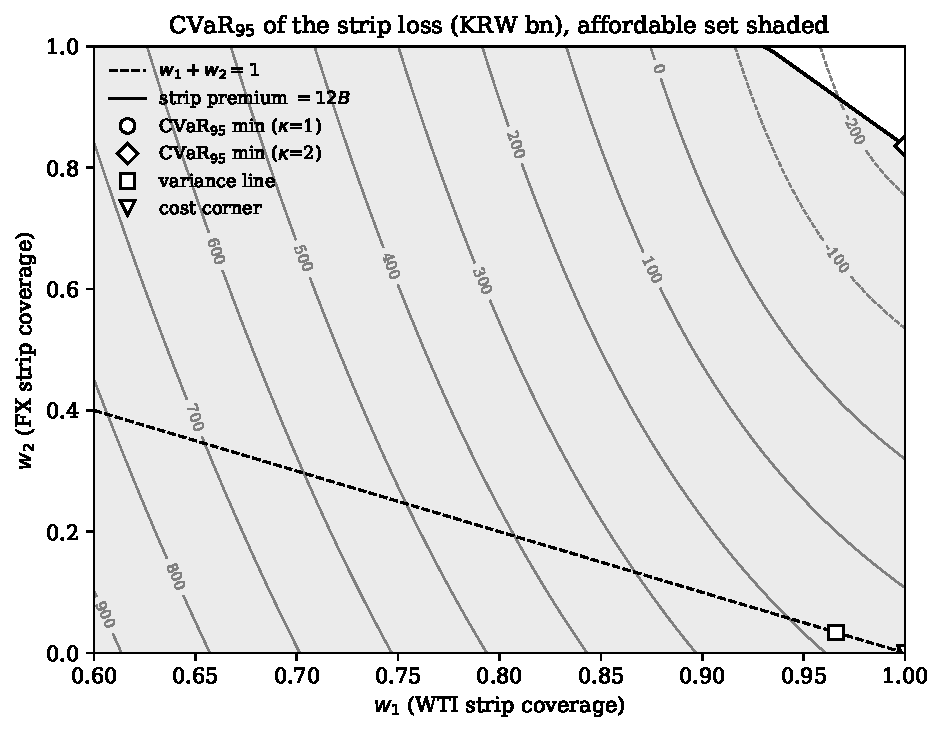
\includegraphics[width=0.85\textwidth]{figures/fig_cvar_contour.pdf}
\caption{CVaR$_{95}$ of the strip loss over the coverage square (KRW bn), with the affordable set $\Pi\le12B$ shaded, the envelope $w_1+w_2=1$ dashed, and the premium boundary solid. The $\kappa=1$ optimum sits at the corner $(1,0)$, coincident with the cost corner; the $\kappa=2$ optimum sits on the premium boundary at $(1,\,0.836)$; the variance-line solution $(0.9660,\,0.0340)$ sits on the envelope.}
\label{fig:cvarcontour}
\end{figure}

\subsection{Question (a): Where the Authority Binds}
\label{sec:binding}

The strip authority's role is decided by the envelope design, and the two designs give opposite answers with a common geometry.

\emph{Under one envelope ($\kappa=1$) the authority is slack everywhere.} The most expensive feasible book is full WTI coverage at KRW 399.8bn, KRW 140.2bn inside the authority; every point on or below the envelope is affordable. The binding constraint at the tail optimum is the envelope itself, and money is not the scarce resource. The same holds for the variance and stress-ledger programs, whose common optimum spends KRW 391.9bn.

\emph{Under separate books ($\kappa=2$) the authority binds exactly.} The tail objective is monotone decreasing in both coverages over the affordable set, so the optimum sits on the premium boundary: $w_1=1$ and $w_2=(12B-K_1^S)/K_2^S=0.8361$, spending the full authority. The last $16.4\%$ of FX coverage, KRW 27.5bn of premium, is the only coverage in the whole program that money excludes. Figure~\ref{fig:authsweep} traces the optimal tail as the authority sweeps from KRW 300bn to 700bn: the $\kappa=1$ curve flattens at KRW 399.8bn, beyond which additional authority buys nothing, while the $\kappa=2$ curve falls at KRW 2.6bn of CVaR$_{95}$ per billion of authority through the KRW 540bn point and flattens only at the full-coverage premium KRW 567.5bn. An authority KRW 27.5bn larger would complete the currency book; the marginal value of that authority, KRW 2.6 of tail per won, is the number a treasury committee needs to price the request.

\begin{figure}[h]
\centering
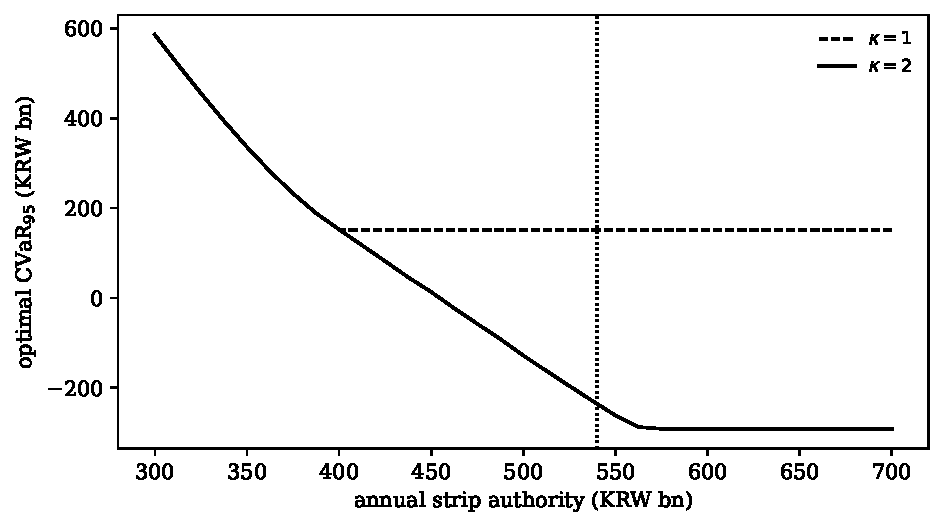
\includegraphics[width=0.8\textwidth]{figures/fig_budget_sweep_strip.pdf}
\caption{Authority sweep. Optimal CVaR$_{95}$ against the annual strip authority under the two envelope designs. The $\kappa=1$ curve flattens at the full-WTI-strip premium (KRW 399.8bn); the $\kappa=2$ curve falls at $\approx$ KRW 2.6bn per billion through the KRW 540bn authority (dotted) and flattens at the full-coverage premium (KRW 567.5bn).}
\label{fig:authsweep}
\end{figure}

\subsection{Question (b): The Asymmetry, in Closed Form and in the Tail}
\label{sec:asymmetry}

\emph{The variance mechanism.} Because $\sigma_{res}$ is strictly decreasing in both coverages, the variance optimum exhausts the envelope, and on the line $w_1+w_2=1$ the problem is the classical two-asset minimum-variance program in the unhedged weights, with closed-form solution
\begin{equation}
w_1^{line} \;=\; \frac{\sigma_1^2 - \rho\,\sigma_1\sigma_2}{\sigma_1^2 + \sigma_2^2 - 2\rho\,\sigma_1\sigma_2}
\;=\; 0.9660.
\label{eq:linegmvp}
\end{equation}
Equation \eqref{eq:linegmvp} \emph{is} the asymmetry: with a variance ratio $\sigma_1^2/\sigma_2^2=18.2$ and correlation $0.0876$, no optimizer on the envelope can choose anything but $w_2=0.0340$. The residual FX openness is the minimum-variance split of one notional envelope across an 18-to-1 variance mismatch at near-zero correlation, and it reads no contract parameter: it is invariant to the strip's maturities, strikes, and premiums.

\emph{The tail mechanism.}
\label{sec:tail}
The tail objective pushes the same asymmetry to its corner, for a reason the variance metric cannot see. The WTI leg's payoff in \eqref{eq:loss} is $(S_1-K_1)^+S_2$: each barrel call settles in dollars converted at the \emph{realized} exchange rate, so on the joint-tail paths where oil spikes and the won depreciates together, the WTI leg's payout is itself inflated by the depreciation. The instrument covers both dimensions of the tail event at once. The FX call's marginal tail contribution, on paths where the WTI leg is already paying, is confined to the currency exposure of the strike leg, and under one envelope every unit of $w_2$ costs a unit of $w_1$ covering eighteen times the variance. The CVaR$_{95}$ optimum at $\kappa=1$ is accordingly the corner $(1,0)$, and it coincides with the cost-minimizing corner: under a tail objective with one envelope, risk minimization and cost minimization select the same book, and the tension between them that the variance benchmark exhibits (its line solution spends KRW 7.9bn less than the corner and carries KRW 25.9bn more tail) is a property of the variance metric, not of the economics.

Released from the envelope at $\kappa=2$, the tail objective does buy currency coverage, KRW 140.2bn of slack authority's worth: the residual FX exposure of a fully covered WTI book is the strike leg $Q_{oil}K_1$ per month, a won liability of KRW 243bn monthly scale whose depreciation risk only FX options can remove, and the optimizer spends the entire remaining authority on it. The asymmetry is therefore a statement about the envelope, at every risk metric: within one notional the barrel dominates; across two notionals the currency book is worth the whole residual authority.

\subsection{Robustness: Correlation and Drift}
\label{sec:robust}

The corner structure makes the allocation robust where an interior solution would be fragile. Re-simulating the bank at $\rho\in\{0.0876,\,0.20,\,0.30,\,0.50\}$, from the sample estimate toward the elevated co-movement documented in stressed regimes by Longin and Solnik (2001) and Ang and Chen (2002), leaves both optima unmoved over this range: the $\kappa=1$ optimum is $(1,0)$ and the $\kappa=2$ optimum is $(1,\,0.836)$ at every $\rho$, the former because the WTI leg's realized-rate settlement covers whatever the correlation couples, the latter because the budget pin is a price fact, not a risk fact. What moves is the level: the $\kappa=1$ tail rises from KRW 151.4bn to 180.2bn as $\rho$ rises to $0.50$, a $19\%$ deterioration carried entirely by the tail the corner book cannot remove, while the $\kappa=2$ tail moves KRW 5.0bn on the same sweep. Over the tested range, correlation risk moves the level of the tail rather than the allocation, and the $\kappa=2$ design absorbs most of the movement. The variance-line solution \eqref{eq:linegmvp}, by contrast, migrates with $\rho$ (to $w_1=0.9770$ at $\rho=0.1376$), which is the familiar fragility of interior minimum-variance weights to correlation error; the tail program's corner structure removes that channel. Replacing the flat-forward FX drift with the uncovered-interest-parity drift $r_{KRW}-r_{US}=-0.005$ moves the $\kappa=1$ tail to KRW 142.9bn and neither optimum.

\subsection{Question (c): The Currency Leg's Maturity}
\label{sec:fxmat}

Each FX slice can be struck at its own settlement date $T_m$ (co-termed) or capped at the half-year tenor, $T^{FX}_m=\min(T_m,\,0.5)$, with slices seven through twelve holding the $0.5$-year option and standing uncovered from its expiry to their settlement. The cap is the configuration a desk reaches for when long-dated FX spreads look forbidding, and the spread curve \eqref{eq:spread} prices exactly that concern: at $s_{1M}=0.4$ vol points and $\gamma=0.5$ the one-year spread is $1.4$ vol points, and at the outer corner of the grid ($s_{1M}=0.8$, $\gamma=1.0$) it is $9.6$.

Evaluated at the $\kappa=2$ optimum, where the currency book is actually held ($w_2=0.836$), the comparison favors the co-termed design by a wide margin (Figure~\ref{fig:fxmat}). The cap's entire economy, cheaper mid premiums on the shortened slices plus the avoided long-tenor half-spreads, ranges from KRW 6.1bn to 14.1bn per year across the whole spread grid. Its cost is the tail it uncovers: capping the six long slices raises the strip's CVaR$_{95}$ by KRW 77.0bn at the same coverage, because the paths on which the currency book matters are exactly the paths on which the depreciation extends past mid-year into the second half's settlements. The cap buys at most KRW 14bn with KRW 77bn; the break-even spread curve sits a further factor of five beyond the steepest curve in the grid. The currency leg belongs at the maturity of the barrels it converts, and the strip's co-termed design is retained throughout this paper.

\begin{figure}[h]
\centering
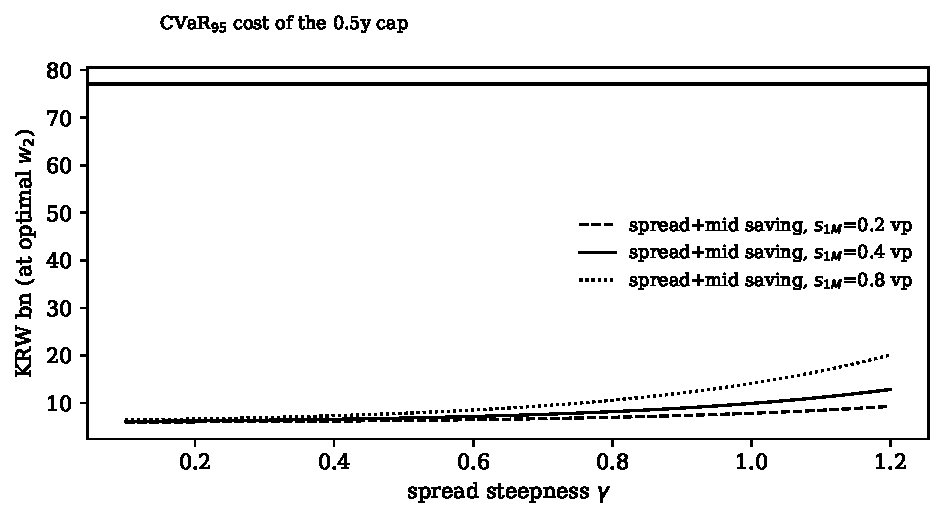
\includegraphics[width=0.8\textwidth]{figures/fig_fx_maturity.pdf}
\caption{The FX maturity decision at the $\kappa=2$ optimum. Curves: annual premium-plus-spread saving of capping FX slices at $T=0.5$, across the spread grid \eqref{eq:spread}. Horizontal line: the CVaR$_{95}$ cost of the cap, KRW 77.0bn, at the same coverage. The saving does not approach the cost anywhere in the plausible region.}
\label{fig:fxmat}
\end{figure}

\section{Survival Adjustment of the Knock-Out Structure}
\label{sec:pko}

This section and the next answer question~(d) at the slice level, on the longest slice ($T=0.833$), where the barrier structure's premium discount is largest and the instrument choice is sharpest; the indifference thresholds derived below are ratios of per-barrel prices and carry to every slice. The candidate instrument is the production knock-out structure: an at-the-money WTI call ($K=78.94$) that dies if WTI trades outside the 120/50 barriers before maturity, priced by LSMC at KRW 33.43bn for the slice against KRW 41.26bn for the same coverage in Black-76 vanillas, against the slice's authority share $B=$ KRW 45bn.

The stress ledger prices the unhedged fraction at the stress scenario while treating the hedged fraction as protected there. For a knock-out structure that treatment fails in precisely the scenario that matters: at the stress price of 113 the upper barrier at 120 is $6.2\%$ away, and a knocked-out call protects nothing. Let $p_{KO}$ be the probability that the structure is dead under the stress scenario. The protected fraction of the leg is then $w_1(1-p_{KO})$, and the survival-adjusted slice ledger becomes
\begin{equation}
\widetilde C(w_1,w_2;\,p_{KO}) \;=\; \text{premiums} \;+\; \bigl(1-w_1(1-p_{KO})\bigr)\,UL_{WTI} \;+\; (1-w_2)\,UL_{FX},
\label{eq:sadj}
\end{equation}
with $UL_{WTI}=Q_{oil}\max(0,113-78.94)\times1550=$ KRW 105.59bn and $UL_{FX}=$ KRW 1.48bn the slice's full-exposure stress losses.

\emph{Two structural thresholds follow in closed form.} While the coefficient on $w_1$ in \eqref{eq:sadj} is negative, the cheapest attainable survival-adjusted ledger is $C(1,0)+p_{KO}\,UL_{WTI}$, which crosses the slice authority at
\begin{equation}
p_{KO}^* \;=\; \frac{B - C(1,0)}{UL_{WTI}} \;=\; \frac{45{,}000{,}000{,}000 - 33{,}425{,}495{,}704}{105{,}586{,}000{,}000} \;=\; 0.1096 :
\label{eq:pstar}
\end{equation}
beyond an $11\%$ stress knock-out probability, no allocation keeps the survival-adjusted ledger within the authority, because the loss floor $p_{KO}\,UL_{WTI}$ is allocation-invariant: the loss floor arises from the knock-out of the same instrument that would otherwise cover it. The coefficient on $w_1$ changes sign at
\begin{equation}
p_{KO}^{\dagger} \;=\; 1-\frac{Q_{oil}\,P^{Sh}_{WTI}\,(1+r_wT_1)}{UL_{WTI}} \;=\; 0.6974,
\label{eq:pdagger}
\end{equation}
above which buying coverage no longer pays for itself against the survival-adjusted stress loss; between the two thresholds the minimizer stays on the $(1,0)$ branch, and Figure~\ref{fig:pko} plots the branch-correct curve throughout.

\emph{The measurement.} Two mortality figures answer two different questions, and both are measured on the calibrated jump-diffusion with jump-adapted exact first-passage sampling at $200{,}000$ paths. A contract \emph{newly struck at the stress spot}, with the barrier $6.2\%$ away and the full $0.833$ years to run, dies with probability
\begin{equation}
p_{KO}^{stress} \;=\; 0.8925 \;\pm\; 0.0007,
\label{eq:pkostress}
\end{equation}
the figure a desk pricing a new structure at the stress spot needs. The importer's question concerns the contract it already holds, struck at $78.94$: conditional on the original contract's path reaching a terminal WTI in the stress band $[108,118]$,
\begin{equation}
p_{KO}^{\,\mathrm{held}} \;=\; 0.4901 \qquad (7{,}992\ \text{of}\ 200{,}000\ \text{paths in the band}),
\label{eq:pkoheld}
\end{equation}
against an unconditional barrier-touch rate of $0.4374$ on the same bank. The held-contract figure is the one the ledger takes, and the two together bracket the range over which the conclusion is tested. The jump calibration underlying \eqref{eq:pkostress} is the asymmetric two-regime fit (up-jumps $\lambda_{up}=2.328$/yr, $\theta_{up}=+8.04\%$, $\delta_{up}=1.68\%$; down-jumps $\lambda_{dn}=4.462$/yr, $\theta_{dn}=-8.75\%$, $\delta_{dn}=2.78\%$); re-deriving it under the symmetrized pool the pricing engines consume gives $0.8937\pm0.0007$, a tenth of a percentage point away, because the $32.4\%$ diffusive volatility dominates barrier-touch dynamics over a sub-annual horizon.

Both measurements sit far above both thresholds. At $p_{KO}^{\,\mathrm{held}}=0.4901$ the all-KO slice ledger reads KRW 86.04bn against the KRW 45bn authority share, $4.5$ times the infeasibility threshold \eqref{eq:pstar}; at $p_{KO}^{stress}$ it reads KRW 127.10bn. Under the scenario the hedge is sized against, an all-KO book provides no protection on roughly half the paths that reach it. The allocation program of Section~\ref{sec:problem} keeps the plain premium constraint \eqref{eq:authority} rather than \eqref{eq:sadj} because the floor $p_{KO}\,UL_{WTI}$ is allocation-invariant; what can respond to \eqref{eq:sadj} is the choice of instrument, which is the degree of freedom the next section adds.

\begin{figure}[h]
\centering
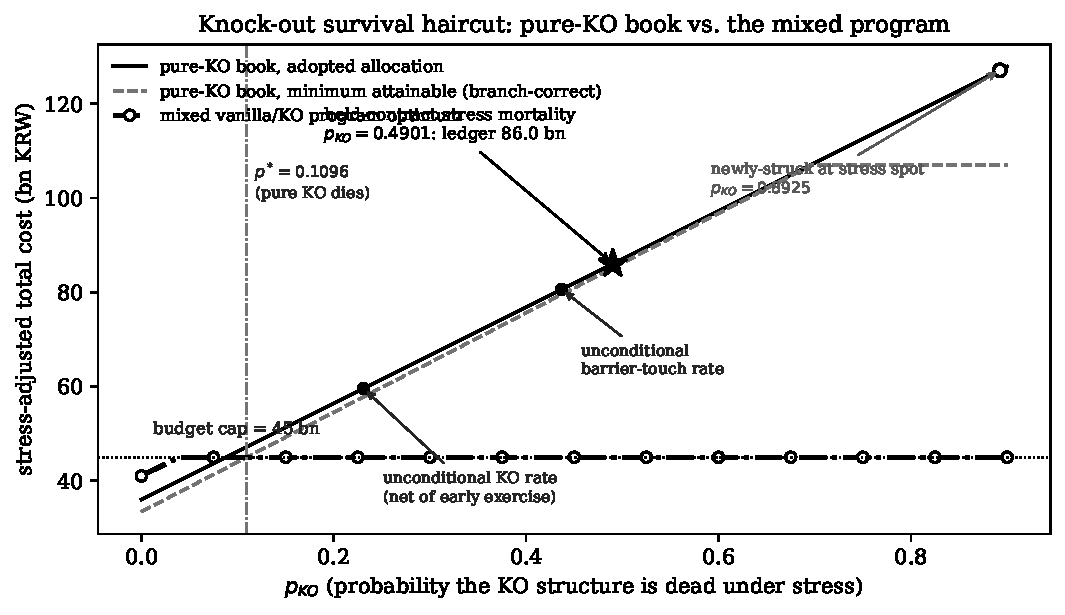
\includegraphics[width=0.8\textwidth]{figures/fig_pko_haircut.pdf}
\caption{Survival-adjusted slice ledger as a function of the stress knock-out probability $p_{KO}$: the pure-KO book at the adopted allocation (solid) and at its cheapest attainable allocation (dashed), against the mixed vanilla/KO program of Section~\ref{sec:mixed} (dash-dotted), which is ledger-feasible for every $p_{KO}$. The dashed curve switches branch at $p^{\dagger}_{KO}=0.6974$ \eqref{eq:pdagger}. Small markers: unconditional knock-out statistics. Star: the stress-spot measurement \eqref{eq:pkostress}. The held-contract mortality \eqref{eq:pkoheld} of $0.4901$ sits at KRW 86.1bn.}
\label{fig:pko}
\end{figure}

\section{The Mixed Vanilla/Knock-Out Program}
\label{sec:mixed}

The survival adjustment treats the instrument as given; this section lets the optimizer choose it along with the coverage. The slice's WTI book is split as $w_1 = w_1^V + w_1^K$ between a vanilla Black-76 leg, which survives stress, and an independently-priced KO leg, which dies with probability $p_{KO}$; the FX leg is priced with the vanilla Garman---Kohlhagen premium; and the survival-adjusted ledger becomes the budget constraint:
\begin{equation}
\min_{w_1^V,\,w_1^K,\,w_2}\ \sigma_{res}(w_1^V{+}w_1^K,\,w_2)
\quad\text{s.t.}\quad
\widetilde C^{mix} \;\le\; B,\qquad w_1^V+w_1^K+w_2\le 1,\ \ w\ge0,
\label{eq:mixprog}
\end{equation}
\begin{equation}
\widetilde C^{mix} \;=\; P_V(w_1^V) + P_K(w_1^K) + P_{GK}(w_2)
+ \bigl(1 - w_1^V - w_1^K(1-p_{KO})\bigr) UL_{WTI} + (1-w_2)\, UL_{FX}.
\label{eq:mixledger}
\end{equation}

The KO leg's premium here is \emph{not} the Shapley-attributed share of the jointly-priced structure: the attribution is a cost-reporting convention for an indivisible instrument (Section~\ref{sec:split}), and the mixed program buys a standalone, separately-tradable KO leg. An independent single-asset LSMC American KO call, priced with no FX coupling on $200{,}000$ jump-adapted exact-first-passage paths, comes to $P_K = $ KRW 17{,}377.11/bbl, $15.1\%$ above the attributed share, and every number in this section uses that standalone price. Both premiums are cash at inception, carried on the same funding factor.

\emph{The split is bang-bang, with a closed-form indifference point.} At any fixed total coverage, \eqref{eq:mixledger} is affine in the split, so its two marginal costs are constants:
\begin{equation}
\frac{\partial \widetilde C^{mix}}{\partial w_1^K} = P_K - (1-p_{KO})\,UL_{WTI}, \qquad\qquad \frac{\partial \widetilde C^{mix}}{\partial w_1^V} = P_V - UL_{WTI}.
\label{eq:margcost}
\end{equation}
KO coverage costs its premium but removes the stress loss only with survival probability; vanilla coverage removes it with certainty. A linear program's optimal split is a corner, and the corner flips where the marginal costs cross:
\begin{equation}
\bar p \;=\; \frac{P_V - P_K}{UL_{WTI}} \;=\; \frac{41{,}258{,}998{,}746 - 36{,}780{,}738{,}568}{105{,}586{,}000{,}000} \;=\; 0.0424.
\label{eq:pbar}
\end{equation}
Below $\bar p$ the discount outruns its mortality and the book is all-KO; above it the book is all-vanilla. The numerator of \eqref{eq:pbar} compares contracts that differ in strike and pricing model as well as in the barrier; the pure barrier discount, measured on one engine and one path bank with only the barrier switched on and off, is KRW $3.4$--$3.6$bn funded ($1{,}613$--$1{,}687$ KRW/bbl across seeds at $200{,}000$ paths), placing the like-for-like indifference mortality at $\bar p_{\mathrm{engine}}\approx3.3\%$; both figures are carried below.

\emph{The solution has three regimes} (Figure \ref{fig:mixswitch}). For $p_{KO} \le 0.0390$ the all-KO branch leaves the budget slack and the program reaches the unconstrained variance floor. For $0.0390 < p_{KO} < \bar p$ the all-KO branch is budget-pinned. At $\bar p = 0.0424$ the book switches to all-vanilla and stays there, invariant in $p_{KO}$: allocation $(0.9705,\,0.0295)$, ledger KRW 45bn, $\sigma_{res}=0.0916$. The all-vanilla corner costs KRW 42.74bn regardless of $p_{KO}$, so the mixed program is feasible at every mortality level: the infeasibility that kills the pure-KO book above \eqref{eq:pstar} cannot occur. The pure-KO death threshold recomputed at the standalone price is $p^*=0.0638$, above the switch point: the optimizer abandons the KO leg on its economics at $0.0424$, before it becomes unaffordable at $0.0638$, and the interval between the two is the range in which a firm could still buy the knock-out but should not.

At the measured mortalities the comparison is decisive. The held-contract figure $0.4901$ is eleven times $\bar p$ and fifteen times $\bar p_{\mathrm{engine}}$; the mixed program selects the all-vanilla book, and against the pure-KO book at the same mortality its ledger reads KRW 45.00bn versus 130.67bn. The switch costs no variance: the mixed optimum matches the pure-KO optimum's residual volatility, $0.0916$, under a strictly harder constraint. The comparison is conservative, because the variance objective \eqref{eq:gmvp} is instrument-blind, crediting $w_1$ with full protection whichever instrument carries it; crediting the KO leg with survival-adjusted coverage $w_1(1-p_{KO})$ instead raises the all-KO book's residual volatility at the measured mortality from $0.0916$ to $0.372$, against $0.0916$ for the vanilla book, so under a survival-adjusted objective the vanilla structure dominates on both axes. The knock-out's premium discount, KRW 4.48bn on the ledger or KRW 3.5bn like-for-like, is the entire case for the instrument, and \eqref{eq:pbar} prices that case at $4.24\%$ of stress mortality against a measured $49\%$.

\begin{figure}[h]
\centering
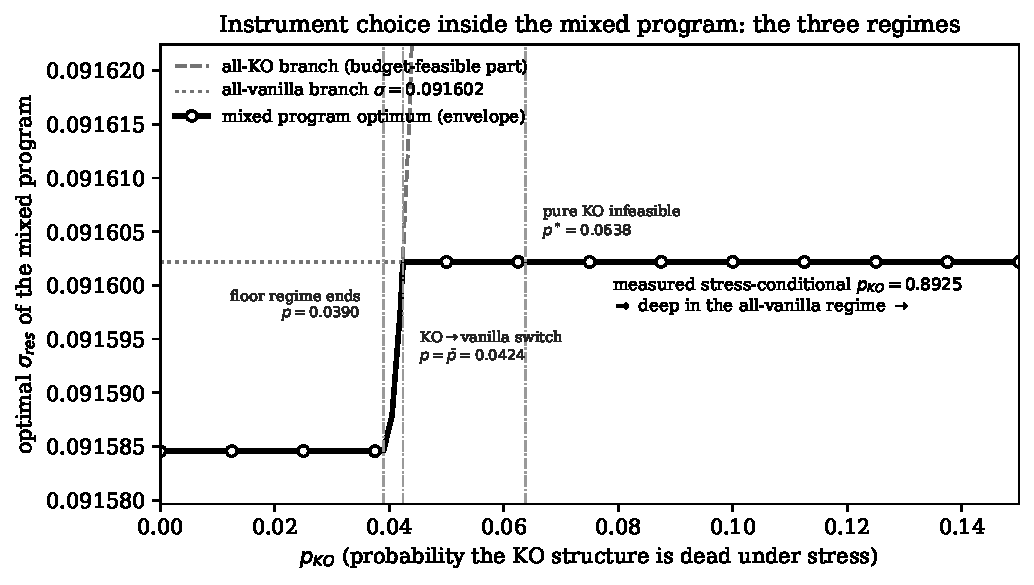
\includegraphics[width=0.8\textwidth]{figures/fig_mixed_switch.pdf}
\caption{The mixed program's optimal residual volatility as a function of $p_{KO}$, at the standalone KO premium. Floor regime ($p_{KO}\le0.0390$): the all-KO ledger leaves the budget slack and the unconstrained variance floor $\sigma_{res}=0.091585$ is attained. Budget-pinned KO regime ($0.0390$---$0.0424$): achieved risk deteriorates as mortality consumes the ledger. All-vanilla regime ($p_{KO}\ge\bar p=0.0424$): the book switches instruments and the optimum is invariant at $\sigma_{res}=0.091602$. The held-contract stress mortality $0.4901$ lies far inside the vanilla regime. The vertical axis is scaled to the $1.8\times10^{-5}$ band the whole switch occupies; on a conventional axis the two levels are indistinguishable, which is the substance of the result: the instrument switch costs essentially no variance.}
\label{fig:mixswitch}
\end{figure}

\section{Discussion}
\label{sec:discussion}

\emph{Maturity matching yields the largest cost saving in the program.} The strip saves KRW 95.3bn per year of WTI premium relative to uniform ten-month contracts, $19.3\%$ of the uniform-tenor cost, before any allocation decision is made. The saving is pure specification: the same coverage of the same exposures, bought without paying for optionality beyond each exposure's life. It also resolves the governance ambiguity that a monthly authority creates against multi-month contracts: in the strip, one slice's premium is spent per month in steady state, and the annual authority \eqref{eq:authority} caps exactly the cash paid.

\emph{The coverage envelope, not the authority level, determines the allocation.} Under one envelope the authority is slack and the tail optimum is the corner $(1,0)$; under separate books the authority binds exactly and prices the currency book's completion at KRW 2.6bn of tail per billion. A treasury that regards the two legs as one bill should know that its tail-optimal book is full WTI coverage and nothing else; a treasury that runs separate books should know that the marginal use of authority is FX coverage, and that KRW 27.5bn more would complete it. Both statements are auditable: the first is a corner of the affordable set, the second a point on its boundary with a computed shadow price.

\emph{The tail and variance objectives rank the corner allocation differently.} The variance benchmark spends KRW 7.9bn less than the $\kappa=1$ corner and carries KRW 25.9bn more CVaR$_{95}$, because the variance metric prices the FX leg's small orthogonal variance but not the joint-tail coverage embedded in the WTI leg's realized-rate settlement. The quanto character of the barrel calls, incidental under a variance objective, is the decisive fact under a tail objective.

\emph{The currency leg's maturity is a tail decision, not a spread decision.} The half-year cap saves premium and spread in single-digit billions and uncovers KRW 77bn of tail, a ratio the examined spread curves do not approach (Section~\ref{sec:fxmat}). On these measurements, the spread saving does not justify the shorter tenor.

\emph{Premium regimes should be compared on the survival-adjusted ledger, which has a decision attached.} On the plain ledger the knock-out dominates: KRW 33.43bn against 41.26bn for the slice. The discount is bought with mortality, measured at $49\%$ for the contract actually held conditional on reaching the stress region, and the mixed program prices the trade at a single indifference number, $\bar p=4.24\%$ ($3.3\%$ like-for-like): the vanilla premium pays for protection that survives the stress state, the knock-out's discount reflects the probability that its protection does not, and at eleven times the indifference mortality the program selects the vanilla book. The vanilla recommendation sits upstream of any dynamic-hedging question: it decides which contract to buy in the first place. The position that results is a barrier-free WTI call correctly hedged by the matching vanilla delta, so no barrier-delta machinery is required downstream.

\section{Practical Implications}
\label{sec:practical}

For the importer's hedging desk the results reduce to five actionable statements. (1) Buy the strip: match each month's options to that month's settlement. The matching itself saves KRW 95.3bn per year on the WTI leg and makes the monthly authority exact. (2) Under the measured stress mortality of $49\%$, hold the WTI book in the vanilla instrument; the knock-out's discount is worth taking only if stress mortality is believed below $4.24\%$ on the ledger, or $3.3\%$ like-for-like, an order of magnitude under the measurement either way. (3) If the two legs share one notional envelope, cover the barrels fully and buy no FX options: the corner $(1,0)$ is simultaneously the tail optimum and the cost optimum, and it leaves KRW 140.2bn of authority unspent. (4) If the currency book is separate, spend the remaining authority on co-termed FX slices up to $w_2=0.836$, and price any request for more authority at its measured shadow value, KRW 2.6bn of CVaR$_{95}$ per billion, up to the completion premium of KRW 27.5bn. (5) Do not shorten the FX slices to save spread: the cap saves at most KRW 14bn and costs KRW 77bn of tail.

\section{Limitations}
\label{sec:limitations}

The program is static: ratios are fixed once for the year, premium constants are invariant to $(w_1,w_2)$, and subsequent dynamic management of the positions is outside this paper's scope. Market impact of the strip's execution and counterparty credit are outside scope.

\emph{The loss distribution inherits the calibration window.} Volatilities, correlation, and the jump triple are estimated on 2021--2026 daily data; the physical WTI drift $\mu_1=0.139$ is that window's sample mean, and drift uncertainty moves tail levels (Section~\ref{sec:robust} reports the UIP variant at KRW 142.9bn against the baseline 151.4bn at the $\kappa=1$ optimum). The allocation corners are invariant across the reported $\rho$ and drift sweeps; the tail levels are not, and should be read with the sweep ranges rather than at face precision.

\emph{The spread term structure is parameterized, not quoted.} Equation \eqref{eq:spread} spans the plausible range of USD/KRW option spreads on a two-parameter family rather than reproducing a quoted surface; the maturity verdict of Section~\ref{sec:fxmat} rests on a factor-of-five margin at the grid's outer corner, which is the reason a parameterized family suffices for it.

\emph{The risk objective for the instrument comparison is scenario-conditional.} The knock-out thresholds \eqref{eq:pstar}--\eqref{eq:pbar} are priced on the stress ledger at (113, 1550); their levels scale inversely with the assumed stress loss ($\bar p$ moves from $23.8\%$ at a stress WTI of 85 to $2.0\%$ at 150), while the direction of the instrument switch at the measured mortality does not, holding at any stress WTI above 85.

\emph{The variance benchmark's interior solution is correlation-fragile.} The line solution \eqref{eq:linegmvp} moves with $\rho$ ($w_1=0.9770$ at $\rho=0.1376$), a known property of minimum-variance weights under estimation error; the tail program's corner structure is the reason the reported allocations do not share this fragility.

\emph{The spending authority is assumed.} The KRW 45bn monthly figure is an assumption stated as a rule, $18.5\%$ of the monthly procurement outlay at the calibration spot; its level determines where the $\kappa=2$ boundary pin \eqref{eq:authority} sits ($w_2=0.836$), and the authority sweep of Figure~\ref{fig:authsweep} reports the allocation at every level from KRW 300bn to 700bn so a treasury operating at a different authority can read its own solution directly.

\section{Conclusion}
\label{sec:conclusion}

A fixed-budget importer choosing WTI and FX hedge coverage faces a program whose maturity structure, risk measure, and instrument set each carry a first-order decision, and this paper prices all three on one calibrated engine. The maturity decision is the cheapest: matching each month's options to its settlement saves KRW 95.3bn per year over uniform-tenor contracts and reconciles the monthly authority with the option book exactly. The allocation decision reduces to the envelope: within one notional envelope the tail-optimal book is full WTI coverage alone, the corner where the tail and cost objectives coincide and the authority is slack, because barrel calls settled at the realized exchange rate cover the joint tail by themselves; across separate books the authority binds exactly, pinning FX coverage at $0.836$ with a shadow price of KRW 2.6bn of CVaR$_{95}$ per billion of authority. Both corners are unchanged over the correlation range examined ($\rho$ up to $0.50$); the closed-form variance split \eqref{eq:linegmvp}, the classical benchmark, is not. The currency leg belongs at the maturity of the barrels it converts: shortening it saves single-digit billions of premium and spread against KRW 77bn of tail across the examined spread curves. The instrument decision is priced by mortality: the knock-out structure is extinguished on half the paths that reach the scenario it is bought against, eleven times the closed-form indifference mortality at which its discount is offset, so the mixed program holds the vanilla book at no cost in residual risk. The static allocation question that precedes every dynamic hedging choice has, for this importer, an answer that is asymmetric, instrument-aware, and maturity-matched, with each margin priced within the stated calibration.

\paragraph{Code and data availability.} Every engine, the frozen derived inputs, and the scripts that regenerate each table and figure in this paper are available at \url{github.com/JihongParker/wti-fx-hedge-program}.

\begin{thebibliography}{9}

\bibitem{adler1984} Adler, M., and B. Dumas (1984). ``Exposure to Currency Risk: Definition and Measurement.'' \emph{Financial Management} 13(2), 41---50.

\bibitem{ahn1999} Ahn, D.-H., J. Boudoukh, M. Richardson, and R. F. Whitelaw (1999). ``Optimal Risk Management Using Options.'' \emph{Journal of Finance} 54(1), 359--375.

\bibitem{anderson1981} Anderson, R. W., and J.-P. Danthine (1981). ``Cross Hedging.'' \emph{Journal of Political Economy} 89(6), 1182---1196.

\bibitem{angchen2002} Ang, A., and J. Chen (2002). ``Asymmetric Correlations of Equity Portfolios.'' \emph{Journal of Financial Economics} 63(3), 443--494.

\bibitem{artzner1999} Artzner, P., F. Delbaen, J.-M. Eber, and D. Heath (1999). ``Coherent Measures of Risk.'' \emph{Mathematical Finance} 9(3), 203--228.

\bibitem{bental1998} Ben-Tal, A., and A. Nemirovski (1998). ``Robust Convex Optimization.'' \emph{Mathematics of Operations Research} 23(4), 769--805.

\bibitem{black1976} Black, F. (1976). ``The Pricing of Commodity Contracts.'' \emph{Journal of Financial Economics} 3(1---2), 167---179.

\bibitem{browntoft2002} Brown, G. W., and K. B. Toft (2002). ``How Firms Should Hedge.'' \emph{Review of Financial Studies} 15(4), 1283--1324.

\bibitem{campello2011} Campello, M., C. Lin, Y. Ma, and H. Zou (2011). ``The Real and Financial Implications of Corporate Hedging.'' \emph{Journal of Finance} 66(5), 1615--1647.

\bibitem{carrchou1997} Carr, P., and A. Chou (1997). ``Breaking Barriers.'' \emph{Risk} 10(9), 139--145.

\bibitem{chopraziemba1993} Chopra, V. K., and W. T. Ziemba (1993). ``The Effect of Errors in Means, Variances, and Covariances on Optimal Portfolio Choice.'' \emph{Journal of Portfolio Management} 19(2), 6--11.

\bibitem{demiguel2009} DeMiguel, V., L. Garlappi, and R. Uppal (2009). ``Optimal Versus Naive Diversification: How Inefficient Is the 1/N Portfolio Strategy?'' \emph{Review of Financial Studies} 22(5), 1915--1953.

\bibitem{derman1995} Derman, E., D. Ergener, and I. Kani (1995). ``Static Options Replication.'' \emph{Journal of Derivatives} 2(4), 78--95.

\bibitem{ederington1979} Ederington, L. H. (1979). ``The Hedging Performance of the New Futures Markets.'' \emph{Journal of Finance} 34(1), 157---170.

\bibitem{froot1993} Froot, K. A., D. S. Scharfstein, and J. C. Stein (1993). ``Risk Management: Coordinating Corporate Investment and Financing Policies.'' \emph{Journal of Finance} 48(5), 1629---1658.

\bibitem{garman1983} Garman, M. B., and S. W. Kohlhagen (1983). ``Foreign Currency Option Values.'' \emph{Journal of International Money and Finance} 2(3), 231---237.

\bibitem{gilje2017} Gilje, E. P., and J. P. Taillard (2017). ``Does Hedging Affect Firm Value? Evidence from a Natural Experiment.'' \emph{Review of Financial Studies} 30(12), 4083--4132.

\bibitem{goldfarb2003} Goldfarb, D., and G. Iyengar (2003). ``Robust Portfolio Selection Problems.'' \emph{Mathematics of Operations Research} 28(1), 1--38.

\bibitem{jinjorion2006} Jin, Y., and P. Jorion (2006). ``Firm Value and Hedging: Evidence from U.S. Oil and Gas Producers.'' \emph{Journal of Finance} 61(2), 893---919.

\bibitem{longinsolnik2001} Longin, F., and B. Solnik (2001). ``Extreme Correlation of International Equity Markets.'' \emph{Journal of Finance} 56(2), 649--676.

\bibitem{longstaff2001} Longstaff, F. A., and E. S. Schwartz (2001). ``Valuing American Options by Simulation: A Simple Least-Squares Approach.'' \emph{Review of Financial Studies} 14(1), 113---147.

\bibitem{maillard2010} Maillard, S., T. Roncalli, and J. Teiletche (2010). ``The Properties of Equally Weighted Risk Contribution Portfolios.'' \emph{Journal of Portfolio Management} 36(4), 60--70.

\bibitem{markowitz1952} Markowitz, H. (1952). ``Portfolio Selection.'' \emph{Journal of Finance} 7(1), 77---91.

\bibitem{merton1976} Merton, R. C. (1976). ``Option Pricing When Underlying Stock Returns Are Discontinuous.'' \emph{Journal of Financial Economics} 3(1---2), 125---144.

\bibitem{michaud1989} Michaud, R. O. (1989). ``The Markowitz Optimization Enigma: Is Optimized Optimal?'' \emph{Financial Analysts Journal} 45(1), 31--42.


\bibitem{perezgonzalez2013} P\'erez-Gonz\'alez, F., and H. Yun (2013). ``Risk Management and Firm Value: Evidence from Weather Derivatives.'' \emph{Journal of Finance} 68(5), 2143--2176.

\bibitem{rampini2014} Rampini, A. A., A. Sufi, and S. Viswanathan (2014). ``Dynamic Risk Management.'' \emph{Journal of Financial Economics} 111(2), 271--296.

\bibitem{reiner1992} Reiner, E. (1992). ``Quanto Mechanics.'' \emph{Risk} 5(3), 59---63.

\bibitem{rockafellar2000} Rockafellar, R. T., and S. Uryasev (2000). ``Optimization of Conditional Value-at-Risk.'' \emph{Journal of Risk} 2(3), 21--41.

\bibitem{roncalli2013} Roncalli, T. (2013). \emph{Introduction to Risk Parity and Budgeting}. Chapman \& Hall/CRC.

\bibitem{shapley1953} Shapley, L. S. (1953). ``A Value for $n$-Person Games.'' In \emph{Contributions to the Theory of Games II}, Princeton University Press, 307---317.

\bibitem{stulz1996} Stulz, R. M. (1996). ``Rethinking Risk Management.'' \emph{Journal of Applied Corporate Finance} 9(3), 8---25.

\end{thebibliography}

\end{document}
